\chapter{Bevezetés}
Ebben a dolgozatban a BME VIK Villamosmérnök MSc képzés Önálló Laboratórium 1 c. tárgyának keretében végzett kutatási és tervezési munkámat összegzem. A dolgozatom témája egy kevéssé ismert nyomtatott antennatípus, a BIFA (Balanced Inverted F Antenna) tervezése.
\section{Kitűzött feladatok}
\section{BIFA}
\par A BIFA antennatípus nem gyakori a szakirodalomban, az irodalomkutatás során csak a Silicon Laboratories egy 2014-es application note-jában \cite{an847} találkoztam vele. Ez az antennatípus egy variációja az IFA-nak (Inverted F Antenna), ezért az IFA jellegzetességeiből kiindulva érdemes tárgyalni.
\begin{figure}[h]
	\centering
	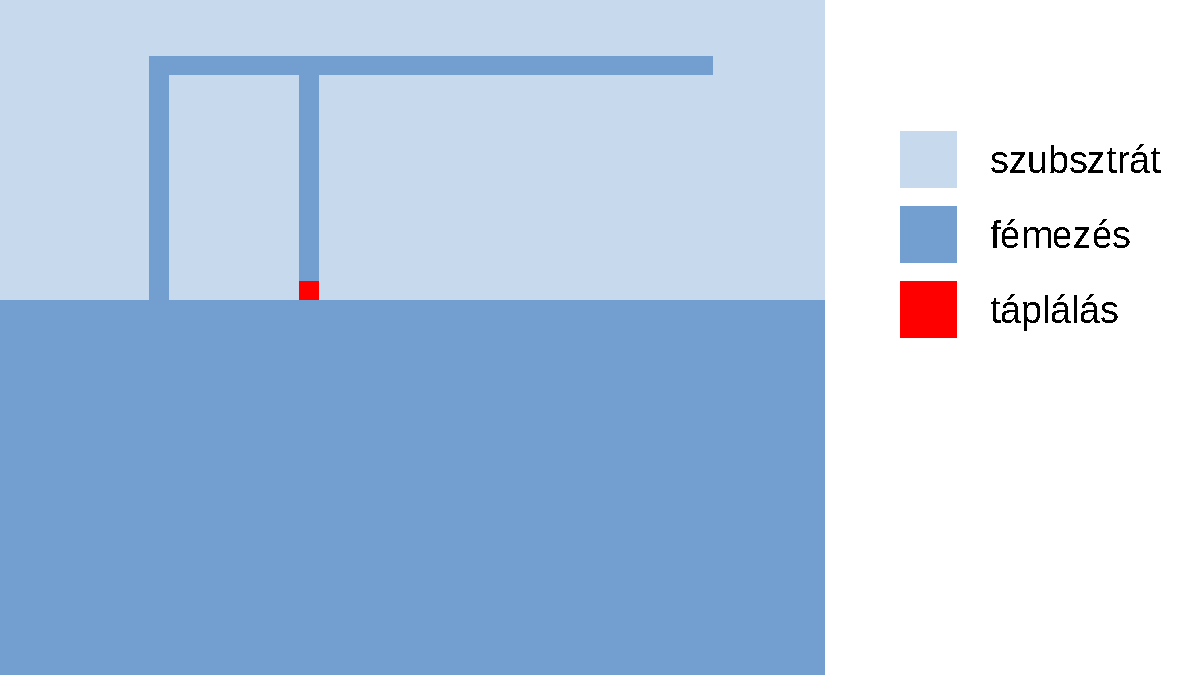
\includegraphics[width=0.7\textwidth]{kep/tipikus_ifa.pdf}
	\caption{Egy tipikus IFA antenna egy nyomtatott áramköri lap szélén.}
	\label{fig:tipikus_ifa}
\end{figure}
\par Az IFA alapvetően egy monopól típusú antenna, emiatt aszimmetrikus táplálású (\ref{fig:tipikus_ifa}. ábra). 
\section{Céges háttér}

